% !TEX encoding = UTF-8
% !TEX TS-program = pdflatex
% !TEX root = ../main.tex
% !TEX spellcheck = it-IT

\documentclass[final, 11pt, a4paper, titlepage]{article}
\makeatletter
\AtBeginDocument{\let\hl\@firstofone}
\makeatother

\usepackage[italian]{babel}
\usepackage[utf8]{inputenc}
\usepackage[hidelinks]{hyperref}
\usepackage{graphicx}
\usepackage{subcaption}
\usepackage{textcomp}
\usepackage{wallpaper}
\usepackage{color}
\usepackage{mathtools}
\usepackage{amssymb}
\usepackage{listings}
\usepackage[
	backend=biber,
	citestyle=numeric-comp,
	hyperref,
	backref,
	sorting=none
]{biblatex}

\graphicspath{{images/}}

\addbibresource{bibliography.bib}


\defbibheading{bibliography}
{
    \phantomsection 
    \addcontentsline{toc}{section}{\bibname}
    \section*{\bibname\markboth{\bibname}{\bibname}}
}

\setlength\bibitemsep{1.5\itemsep} 

%\DeclareBibliographyCategory{sampleCategory}

%\addtocategory{sampleCategory}{referenceID}


\newcommand{\university}{Università degli Studi di Padova}
\newcommand{\dept}{Dipartimento di Matematica}
\newcommand{\faculty}{Laurea Magistrale in Informatica}
\newcommand{\myyear}{Anno Accademico 2016-17}
\renewcommand{\title}{Making Android run on time}
\newcommand{\subtitle}{Relazione}
\renewcommand{\author}{Matteo Di Pirro}
\newcommand{\matr}{1154231}

\begin{document}
	\begin{titlepage}
\begin{center}

\begin{LARGE}
\textbf{\university}\\
\end{LARGE}

\vspace{10pt}

\begin{Large}
\textsc{\dept}\\
\end{Large}

\vspace{10pt}

\begin{large}
\textsc{\faculty}\\
\end{large}

\vspace{30pt}
\begin{figure}[htbp]
\begin{center}

\includegraphics[height=6cm]{images/logo_unipd}
\end{center}
\end{figure}
\vspace{30pt} 

\begin{LARGE}
\begin{center}
\textbf{\title}\\
\end{center}
\end{LARGE}

\begin{Large}
	\begin{center}
		\textbf{\subtitle}\\
	\end{center}
\end{Large}

\vspace{20pt} 

\begin{large}
\begin{flushright}
\textit{\author \\ \matr}
\end{flushright}
\end{large}

\vspace{40pt}

\line(1, 0){338} \\
\begin{normalsize}
\textsc{\myyear}
\end{normalsize}

\end{center}
\end{titlepage} 
	\tableofcontents
	\newpage
	\section{Java per sistemi real-time}
L'uso di Java per sistemi real-time non è diffuso per varie ragioni. Le applicazioni Java vengono eseguite su una JVM in un sistema operativo general-purpose che può solo sperare di soddisfare requisiti di response time nell'ordine delle centinaia di millisecondi. Molti aspetti diversi del linguaggio sono responsabili di questi ritardi: la gestione dei thread, il caricamento dinamico delle classi, la compilazione Just-in-Time (JIT) e la garbage collection (GC). Alcune di questi effetti possono essere mitigati in fase di progettazione, ma solo con moltissimi sforzi. 

\subsection{Gestione dei thread}
Java non dà nessuna garanzia sullo scheduling o sull'utilizzo di priorità. Un'applicazione che deve rispondere agli eventi in un tempo ben definito non ha nessun modo di assicurare che un thread a bassa priorità non venga eseguito al posto di uno con priorità più alta. Per compensare, un programmatore dovrebbe dividere l'applicazione in ''sotto-applicazioni'' e farle eseguire a diverse priorità. Questo partizionamento, tuttavia, comporta una maggiore difficoltà di comunicazione e un overhead aggiuntivo.

\subsection{Caricamento dinamico delle classi}
Una JVM che rispetti la specifica di Java deve ritardare il caricamento delle classi fino a quando queste non vengono per la prima volta riferite nel programma. Il caricamento, quando avviene, può richiedere una quantità variabile di tempo, dipendentemente dal supporto fisico (disco o altro) dal quale la classe viene caricata e dalla dimensione. Generalmente il ritardo introdotto è oltre i 10ms. Di conseguenza, se decine o centinaia di classi vengono caricate, il caricamento può portare ad un ritardo significativo. Un design attento può caricare tutte le classi allo start-up, ma questa procedura va fatta manualmente.

\subsection{Garbage Collection}
La garbage collection ha vari benefici rispetto ad applicazioni classiche: pointer safety, leak avoidance e libera i programmatori dal dover gestire la memoria manualmente (tedioso e molto error-prone). Sfortunatamente però la garbage collection viene avviata automanticamente quando lo heap viene esaurito al punto tale che una richiesta di allocazione non può essere esaudita. Anche l'applicazione può chiedere una collection.

La pulizia della memoria avviene tramite la cosiddetta politica \textbf{Stopping the World}. L'applicazione viene messa in pausa per permettere al GC di pulire la memoria. Gli oggetti vivi vengono tracciati a partire da un insieme radice (oggetti puntati da campi statici, oggetti vivi nello stack dei thread, ecc). La memoria che non contiene questi oggetti viene libreata per una futura allocazione. Le pause introdotte dal GC sono illimitate in lunghezza e tipicamente sono molto intrusive (range centinaia di ms a secondi). La durata dipende dalla dimensione dello heap, dal numero di oggetti vivi e dal grado di aggressività del GC. Algoritmi più moderni utilizzano tecniche concorrenti o incrementali per ridurre il tempo di pausa, ma anche con queste tecniche non esiste un limite fissato alle attività di pulizia.

Se da un lato il non doversi preoccupare della gestione della memoria è un grande vantaggio, dall'altro la GC può introdurre pesanti ritardi, impossibili da prevedere staticamente. L'unica soluzione al problema è non usare affatto la GC, ma non è una soluzione praticabile sia per la complessità del codice da gestire sia perché difficilmente si possono trovare librerie esterne che non la utilizzano.

\subsection{Compilazione}
La maggior parte delle JVM commerciali compilano in codice nativo le parti dell'applicazione utilizzate più di frequente. Sfortunatamente l'esecuzione di codice compilato o interpretato avviene con tempi anche molto diversi tra loro. Per un'applicazione real-time l'impossibilità di prevedere quando il codice Java verrà compilato in codice nativo introduce troppo non determinismo per poter analizzare i tempi di esecuzione. Una soluzione è compilare a mano una lista di metodi che si sa essere eseguiti di frequente, ma l'operazione è molto error-prone.	
	\begin{frame}{Real-Time specification for Java \\e altre soluzioni}
	\begin{itemize}
		\item Scheduling
		\begin{itemize}
			\item Utilizzo reale delle priorità
			\item Basic Priority Inheritance Protocol
			\item Ceiling Priority Protocol (opzionale)
		\end{itemize}
		\item Gestione della memoria
		\begin{itemize}
			\item Scoped
			\item Immortal
		\end{itemize}
		\item Compilazione Ahead of time
		\begin{itemize}
			\item Maggiore prevedibilità
		\end{itemize}
	\end{itemize}
\end{frame}
	\section{Confronto delle tecniche di compilazione}
Storicamente le performance delle applicazioni Java sono sempre state molto criticate. Java è stato progettato per essere interpretato e portabile: i primi runtime avevano performance significativamente più basse dei concorrenti. Nel corso degli ultimi anni, però, i runtime Java hanno introdotto compilatori dinamici molto sofisticati: i compilatori JIT. Questi compilano selettivamente i metodi più frequentemente eseguiti in codice nativo durante l'esecuzione. Il fatto di compilare i metodi durante l'esecuzione, e non allo start-up, mantiene la portabilità. Grazie a questo, inoltre, le performance risultano incredibilmente migliorate. 

\subsection{Compilazione Just-in-time}
Figura~\ref{fig:jit} mostra un esempio di compilazione just-in-time. 
\begin{figure}
	\centering
	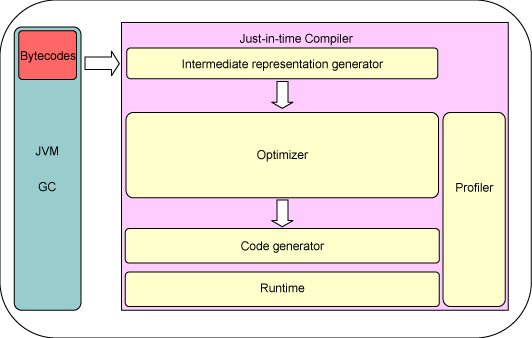
\includegraphics[width=0.7\linewidth]{jvmjit}
	\caption[Compilatore JIT]{Compilatore JIT}
	\label{fig:jit}
\end{figure}
I programmi Java vengono compilati un metodo alla volta mentre eseguono, per raggiungere performance migliori. Durante il processo viene generata una rappresentazione interna del metodo (differente dal bytecode, ma ad un livello più alto delle istruzioni macchina). Il compilatore poi esegue una serie di ottimizzazioni per migliorare la qualità e l'efficienza del codice finale e infine traduce tutto in istruzioni macchina del processore in uso. Il compilatore opera in un thread differente cosicché l'applicazione non è costretta a bloccarsi in attesa della fine della compilazione. Un framework (\texttt{Profile}) osserva il comportamento del programma per identificare i metodi eseguiti più frequentemente. 

L'eseguire la compilazione concorrentemente all'esecuzione mantiene l'indipendenza dalla piattaforma, ma ad un costo: il tempo richiesto per compilare si somma al tempo richiesto per l'esecuzione. Ci sono due soluzioni al problema:
\begin{itemize}
	\item compilare tutto il codice senza però effettuare analisi o ottimizzazioni costose (per mantenere veloce il processo). L'overhead in questo caso è talmente piccolo che è completamente recuperato dall'incremento di performance; 
	\item compilare solo metodi eseguiti veramente frequentemente (metodi \textit{hot}). L'overhead è mantenuto basso perché molte applicazioni eseguono frequentemente solamente una piccola parte del codice, quindi è sufficiente compilare quello per ottenere un significativo aumento di performance.
\end{itemize}

\subsubsection{Vantaggi}
I compilatori JIT possono analizzare l'esecuzione e identificare le situazioni che si avverano più comunemente. A partire da queste possono poi compilare il codice (anche con ottimizzazioni molto spinte) per raggiungere performance altissime. Un esempio è dato da una semplice procedura di copia di un array, \texttt{arrayCopy}. Se viene rilevato che la dimensione dell'array è praticamente costante allora è possibile generare codice ottimizzato per quella lunghezza. 

\subsubsection{Svantaggi}
Dato che è necessaria una fase di ''training'' per capire quali parti compilare, spesso le migliori performance si ottengono dopo un po'. Inoltre i metodi eseguiti frequentemente in questo periodo iniziale potrebbero non essere effettivamente quelli più significativi. Ad ogni modo le tecniche di analisi utilizzate oggigiorno eliminano il problema. 

Alcune applicazioni, però, non possono tollerare il ritardo introdotto dalla compilazione. Un esempio sono quelle da eseguire real-time.

\subsection{Compilazione Ahead-of-time}
La compilazione AOT la trasformazione in codice nativo avviene a priori, prima dell'esecuzione. Questo evita i problemi di analisi del codice e del ritardo di esecuzione, ma introduce altre problematiche. Una di queste è dovuta al caricamento dinamico delle classi. Il compilatore in questo caso non può fare nessuna assunzione riguardo a quali classi saranno caricate. Queste possono risiedere in altre macchine oppure non esistere affatto prima dell'esecuzione (con meccanismi di reflection è possibile creare classi ''al volo'', durante l'esecuzione). Questa è una grande limitazione, perché inibisce alcune delle più importanti ottimizzazioni effettuate dai compilatori, tra cui l'inlining. 

Il codice deve quindi essere generato con tutti i riferimenti non risolti. Durante l'esecuzione ogni riferimento utilizzato è aggiornato con il suo valore reale. Questo può comportare una penalità nella prima esecuzione, perché tutti i riferimenti sono sconosciuti, ma le esecuzioni successive non soffriranno di ritardi.

Compilare tutto il codice può non essere una buona scelta: il codice nativo occupa generalmente più spazio, e molti metodi sono utilizzati così raramente che la loro compilazione non porta benefici. Tuttavia invocare metodi interpretati da metodi compilati (o viceversa) richiede molto più tempo che invocare metodi interpretati da metodi interpretati. Un compilatore JIT può risolvere il problema al volo, ma uno AOT deve selezionare attentamente cosa compilare e cosa no, a priori. 

\subsubsection{Vantaggi}
Il codice AOT, sebbene più lento di quello JIT, è molto più veloce del codice interpretato. Inoltre l'incremento di performance si ottiene più velocemente, perché non si devono compilare al volo metodi eseguiti frequentemente. Le applicazioni real-time, in particolare, traggono numerosi benefici da questo approccio. Le performance sono migliori e più deterministiche rispetto a JIT. 

\subsection{Confronto}
Figura~\ref{fig:performanceaotvsjit} mostra un confronto basato sulle performance. 
\begin{figure}[h]
	\centering
	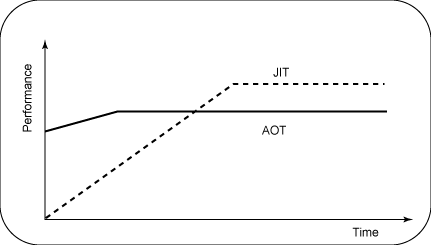
\includegraphics[width=0.7\linewidth]{performanceaotvsjit}
	\caption[Confronto di performance]{Confronto di performance}
	\label{fig:performanceaotvsjit}
\end{figure}

Inizialmente JIT è molto peggiore, perché tutti i metodi sono interpretati. Man mano che vengono compilati però le prestazioni migliorano fino a superare AOT e a raggiungere un picco. AOT, d'altra parte, ha un inizio migliore e si stabilizza più velocemente, ma ad un livello più basso. Nessuna tecnica è adatta per tutti gli scenari: l'una è più forte dove l'altra è più debole. Per le applicazioni real-time, dove l'importante è il determinismo e la prevedibilità, AOT è molto più adatto perché presenta meno variabilità nelle prestazioni.
	\section{Fiji VM}
I linguaggi più utilizzati, in genere, per sistemi real-time sono Ada e C (per i più coraggiosi C++). Tuttavia la complessità e la dimensione crescente del codice, unita alla disponibilità di tanti programmatori ben addestrati hanno portato fatto crescere l'interesse verso l'utilizzo di Java. Inoltre, dato che le applicazioni Android sono generalmente scritte in Java, per poter utilizzare quei dispositivi in contesti con vincoli temporali è necessario avvicinare il mondo Java e quello real-time. Per farlo è necessario sviluppare un runtime, e una GC, che siano prevedibili e adatti all'utilizzo in sistemi con vincoli temporali stretti. La Fiji VM (fVM) ha esattamente questo scopo. Figura\ref{fig:fijiarch} mostra la sua architettura.
\begin{figure}
	\centering
	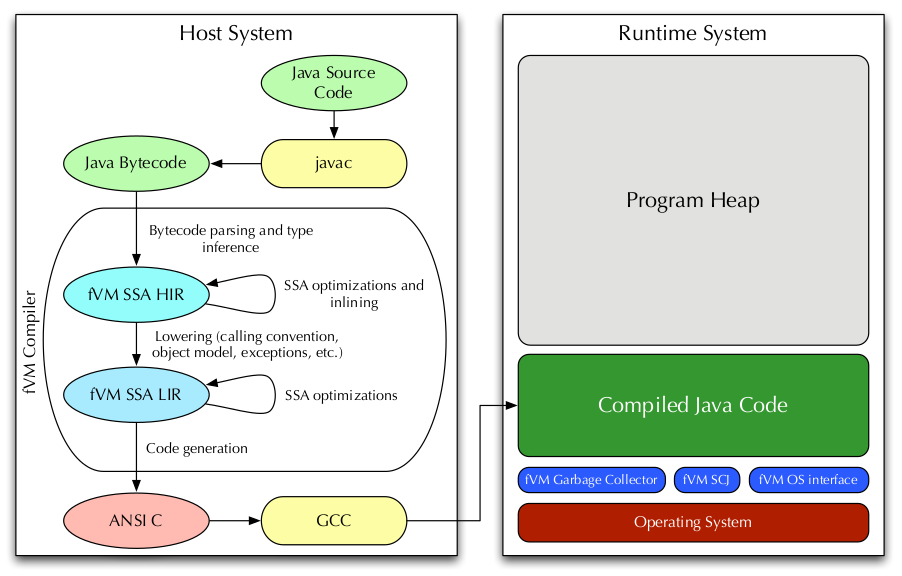
\includegraphics[width=0.9\linewidth]{fijiarch}
	\caption[Architettura di Fiji VM]{Architettura di Fiji VM}
	\label{fig:fijiarch}
\end{figure}

\subsection{Compilazione}
fVM utilizza un compilatore AOT per convertire codice Java in ANSI C. A partire dal codice Java vengono inizialmente effettuate diverse ottimizzazioni basate sulla rappresentazione static-single-assignment (SSA); tra queste troviamo:
\begin{itemize}
	\item inlining;
	\item devirtualizzazione (chiamate virtuali tradotte in chiamate dirette;
	\item virtualizzazione (chiamate di interfaccia in chiamate virtuali);
	\item eliminazione dei lock (se si sa che un lock è attivo non serve fare avere codice che lo attiva nuovamente);
	\item eliminazione dei controlli sulle dimensioni degli array e sui null pointers;
	\item copy propagation.
\end{itemize}
Di seguito vengono descritte le modalità di compilazione.

\paragraph{Null pointers} \mbox{} \\
Java controlla che ogni puntatore sia non null prima di utilizzarlo. Attraverso tecniche di analisi del flusso di controllo è possibile eliminare questi controlli ed evitare percorsi di esecuzione diversi con tempi diversi.

\paragraph{Dimensione degli array} \mbox{} \\
Così come per i controlli sui puntatori nulli, anche i controlli sugli indici degli array possono essere rimossi per evitare di incorrere in incrementi del tempo di esecuzione.

\paragraph{Controlli per la garbage collection} \mbox{} \\
Dato che il GC opera concorrentemente all'applicazione (= non la mette in pausa), è necessario fare alcuni controlli a run-time:
\begin{itemize}
	\item \textbf{sync-points}: indicano che lo stack del thread corrente deve essere analizzato dal GC;
	\item \textbf{stone barriers}: assicurano che le modifiche fatte allo heap siano viste dal GC.
\end{itemize}
I primi sono inseriti utilizzando una politica che assicura una distanza limitata tra due diversi punti. Questo significa che ogni ciclo ne avrà almeno uno. L'impatto sui cicli ''snelli'' è significativo, perché viene introdotto un nuovo branch. Tuttavia i test effettuati mostrano che, in generale, l'overhead è trascurabile. fVM mantiene un puntatore ad una struttura dati corrispondente allo del thread corrente. Questa struttura contiene un campo, \texttt{shouldSync}, che è \texttt{true} quando il thread deve sincronizzarsi (\texttt{yield()}). I thread con alta priorità, tale da poter prerilasciare il GC, non sono affetti da questo controllo, ma tutti gli altri subiranno un overhead inevitabile. 

Le seconde introducono un altro overhead nella pulizia, e vengono tradotte nel modo seguente (per ogni modifica ad un puntatore):
\begin{lstlisting}[caption={Stone-barrier},label={lst:stone}]
if (source != null && source.gcState != marked)
	mark(source);
target.field = source;
\end{lstlisting}
Il primo controllo è spesso rimosso (in virtù di quanto detto prima), ma comunque i due percorsi avranno tempi di esecuzione diversi (rallentamento se la condizione è vera).

\paragraph{Variabili locali} \mbox{} \\
La maggior parte delle assegnazioni di variabili locali sono eliminate attraverso copy propagation o tradotte in assegnazioni C. Questo non vale se le variabili contengono puntatori. Infatti i compilatori C non forniscono metodi adeguati per analizzare lo stack, operazione necessaria per la GC. Il problema viene risolto utilizzando una struttura allocata sullo stack che contiene copie a tutti i riferimenti locali allo heap. In questo modo è possibile sempre avere la situazione dei riferimenti locali sotto controllo, senza impattare significativamente le performance.

\paragraph{Invocazione di metodi} \mbox{} \\
L'invocazione dei metodi è tradotta in una chiamata di funzione C. Ci sono vari overhead indiretti legati alla gestione della struttura dati per la GC e al controllo delle eccezioni. Per ovviare a questi problemi vengono effettuate ottimizzazioni di inlining e devirtualizzazione molto aggressive. I metodi piccoli o quelli chiamati molto spesso (a meno che non siano \textit{troppo} grandi) vengono aggiunti inline. I metodi ricorsivi sono penalizzati, perché l'inlining ricorsivo viene evitato, ma gli altri raggiungono velocità pari agli equivalenti C.

\paragraph{Inizializzazione statica} \mbox{} \\
Java aggiunge controlli sull'inizializzazione delle classi prima di ogni chiamata di un metodo statico, di ogni accesso ad un campo statico e di ogni istanziazione. I controlli ridondanti possono essere rimossi analizzando il flusso di controllo. Le librerie sono state inoltre progettate per fare un uso minimo dell'inizializzazione statica o per permettere alla VM di inizializzare il più possibile prima dell'esecuzione. Tali controlli possono quindi essere rimossi dal compilatore.

\paragraph{Allocazione} \mbox{} \\
Per allocare memoria viene fatto un primo tentativo con del codice C per salvare l'oggetto nella prima posizione raggiungibile. Se l'allocazione fallisce, si cerca la prima posizione disponibile. Il GC agisce in modo concorrente, ma ci possono essere dei casi nei quali l'applicazione è costretta a mettersi in pausa in attesa del completamento della pulizia (se la memoria è piena). L'intera procedura è al più tanto lenta quanto una chiamata C \texttt{malloc}. 

\paragraph{Sincronizzazione} \mbox{} \\
Viene utilizzato codice C per acquisire velocemente il lock e codice specifico per permettere la gestione dei lock rispettando RTSJ. I lock del SO sono utilizzati internamente, e l'implementazione è molto più efficiente rispetto a quella ottenuta utilizzando solamente C.

\subsection{Garbage Collection}
%todo

\subsection{Valutazione}
Figura\ref{fig:fijicomp} mostra un confronto di varie VM progettate per sistemi real-time (fVM e WebSphere) e fortemente ottimizzate (Hotspot). 
\begin{figure}[h]
	\centering
	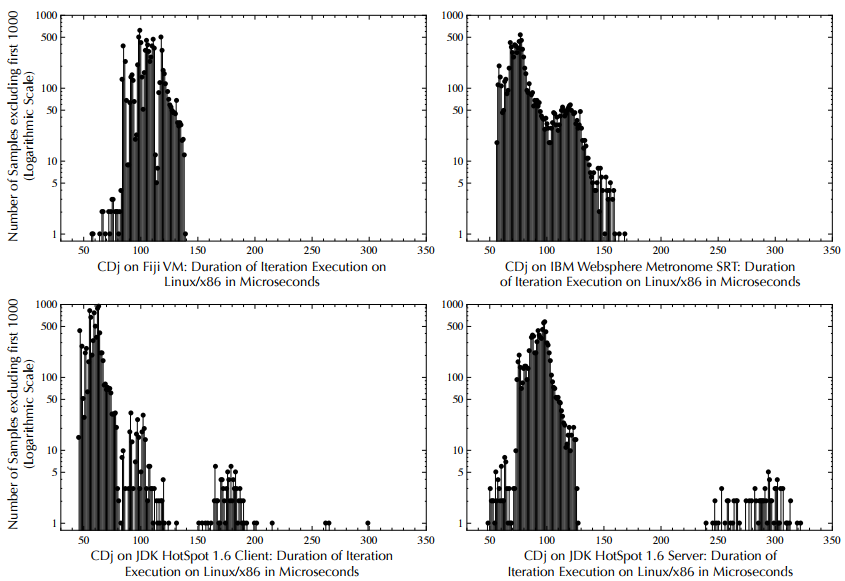
\includegraphics[width=0.8\linewidth]{images/fijicomp}
	\caption[Valutazione rispetto ad altre VM]{Valutazione di FijiVM rispetto ad altre VM}
	\label{fig:fijicomp}
\end{figure}

Si nota che Hotspot è decisamente più veloce rispetto a Fiji (37\% Server e 4.7\% Client), ma nel caso peggiore (quello realmente importante per sistemi real-time), Hotspot si comporta molto male (circa 185/200\% peggio di Fiji). Queste differenze sono causate dalle pause introdotte dalla GC, che non tiene conto della prevedibilità, ma cerca solo di ottimizzare il caso migliore. Rispetto a WebSphere, invece, Fiji si comporta meglio (nel caso peggiore) del 4\%, anche se in generale WebSphere è più veloce del 15\%. Tuttavia Fiji ha una distribuzione più stretta (calcolata rispetto alla differenza picchi/valli). Questo è un grande pregio, perché significa che la differenza tra il caso migliore e quello peggiore è più bassa.

Figura\ref{fig:fijistartup} mostra l'evoluzione del caso peggiore per diverse VM. Il grafico è in qualche modo simile a quello mostrato in Figura\ref{fig:performanceaotvsjit}. Hotspot e WebSphere utilizzano un compilatore JIT. Di conseguenza i tempo necessario al raggiungimento delle migliori prestazioni è variabile e più alto di quello di Fiji, che usa un compilatore AOT. Come detto precedentemente, le performance in generale saranno migliori per le altre VM (confermato da Figura\ref{fig:fijicomp}), ma il tempo necessario per raggiungere quei livelli è alto e riduce il determinismo.
\begin{figure}[h]
	\centering
	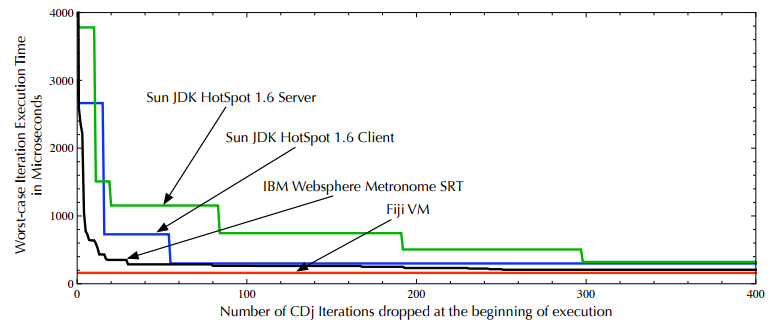
\includegraphics[width=0.8\linewidth]{images/fijistartup}
	\caption[Evoluzione del caso peggiore]{Evoluzione del caso peggiore per diverse VM}
	\label{fig:fijistartup}
\end{figure}

	\section{Prima valutazione sull'utilizzo di Android in contesti real-time}
Fin dalla sua nascita Android ha generato moltissimo interesse intorno a sé. Il fatto di essere open-source gli permette di essere ben studiato e compreso. Inoltre chiunque può provare a fare dei miglioramenti o ad adattarlo in base alle proprie esigenze. Ricercatori e non hanno provato a fondo le funzionalità offerte, portando e proponendo modifiche a vari livelli per scopi diversi: sicurezza, uso nell'industria, ecc. In molti hanno anche studiato la possibilità di utilizzarlo in contesti real-time. 

Tuttavia, Android non è stato pensato per un utilizzo in contesti con seri vincoli temporali. Molte scelte, architetturali e non, lo penalizzano in quest'ottica. Di seguito ne verranno analizzate alcune.

\subsection{Garbage Collection}
Il garbage collector di Android è di tipo stopping-the-world, e non può essere eseguito concorrentemente con l'applicazione. Inoltre, ogni applicazione in esecuzione ha un suo garbage collector. Il runtime controlla lo stato di tutti i thread, e il garbage collector viene eseguito solo quando nessun thread legato ad un processo è in esecuzione. Questo significa che l'applicazione è ferma mentre il runtime pulisce la memoria. La strategia di pulizia è di tipo mark-sweep, con tutti i vantaggi e gli svantaggi discussi nella Sezione~ref{sec:gc}.

\subsection{Scheduler}
Android utilizza lo stesso algoritmo di scheduling del kernel Linux, ovvero \textbf{Completely Fair Scheduling} (CFS), un algoritmo basato sul concetto di virtual clock. Quest'ultimo misura la quantità di tempo di processore che, in un sistema completamente fair, sarebbe stata data ad un processo in attesa. Linux non memorizza questa informazione, ma la calcola a partire da una struttura simile alla seguente:
\begin{lstlisting}[language=c, caption={Entità schedulabile in Linux}, label={lst:schedentity}]
struct sched_entity {
	...
	u64 exec_start;
	u64 sum_exec_runtime;
	u64 vruntime;
	u64 prev_sum_exec_runtime;
	...
}
\end{lstlisting}
Quando un processo è assegnato ad una CPU, \texttt{exec\_start} è aggiornato all'istante attuale e il tempo di esecuzione è memorizzato in \texttt{sum\_exec\_runtime}. Quando il processo lascia la CPU \texttt{sum\_exec\_runtime} viene copiato in \\\texttt{prev\_sum\_exec\_runtime}. \texttt{sum\_exec\_runtime} è calcolato incrementalmente, cioè cresce monotonicamente. Infine, \texttt{vruntime} memorizza l'ammontare di tempo che è trascorso nel virtual clock durante l'esecuzione del processo. Quest'ultimo è incrementato della seguente quantità:
\[ delta\_exec\_weighted = delta\_exec * \frac{NICE\_0\_LOAD}{load.weight}; \]
dove \texttt{delta\_exec} è il tempo di CPU del processo e \texttt{load.weight} è il peso del processo. L'utilizzo a denominatore del peso può essere considerato come un fattore di correzione. Task con alta priorità (e con basso valore nice) avranno peso maggiore. Di conseguenza l'incremento di \texttt{vruntime} sarà piccolo. Run-time virtuale e fisico sono uguali quando per task con $nice = 0$ e priorità 120, cioè quando $load.weight = NICE\_0\_LOAD$. Solitamente un aumento di nice di 1 unità risulta in un tempo di CPU minore di circa 10\%. 

La coda di esecuzione è mantenuta in un albero rosso nero e ogni coda (una per CPU) memorizza un campo \texttt{min\_vruntime}. Quest'ultimo rappresenta il più piccolo \texttt{vruntime} tra tutti i processi nella coda (di conseguenza può solo aumentare, e mai diminuire). Le chiavi per i nodi dell'albero rosso nero sono date da $vruntime - minruntime$, per ogni processo nella coda.

Quando lo scheduler è invocato, il kernel prende il task con la chiave minore (che sarà memorizzato nella posizione più a sinistra), e gli assegna la CPU. Quindi gli elementi con chiave minore sono posizionati più a sinistra, e saranno eseguiti prima.

Quando un processo esegue, il suo \texttt{vruntime} aumenta costantemente, fino a quando non si posizionerà nella parte più a destra dell'albero. Dato che questo campo aumenta più lentamente per i task ad alta priorità, loro si muoveranno verso destra più lentamente. Questo significa che loro hanno più possibilità di essere eseguiti rispetto a quelli a bassa priorità, come è giusto che sia. Se un processo è in attesa il suo \texttt{vruntime} resta inalterato, ma dato che il \texttt{min\_runtime} della cosa aumenta costantemente prima o poi q	uel processo verrà svegliato perché la sua chiave è diventata la minore. 

In questo protocollo non ci sono possibilità di starvation, dato che prima o poi tutti verranno eseguiti. Inoltre, se un task si mette in attesa per I/O verrà ricompensato con tutta la quantità di tempo che è stata necessaria per completare l'operazione. 

Lo scheduler di Linux è modulare e prevede diverse classi di scheduling per poter utilizzare diversi algoritmi/politiche per diverse occasioni. Una classe di scheduling di fatto fornisce un'interfaccia allo scheduler principale per permettere di gestire task usando diversi algoritmi. Come previsto dallo standard POSIX, Linux dispone di due classi soft real-time: \textbf{SCHED\_RR}, per politiche round robin, e \textbf{SCHED\_FIFO}, per politiche FIFO. Android però fa scheduling utilizzando prevalentemente \textbf{SCHED\_OTHER}, che non offre nessun supporto real-time.

Di conseguenza lo scheduling di Android da più importanza alla fairness, una proprietà che non interessa ai sistemi real-time. 

\subsection{Gestione di interruzioni ed eventi}
Il kernel è responsabile di notificare l'applicazione quando arriva un'interruzione o si verifica un evento. Purtroppo però nessuna componente coinvolta in questo meccanismo ha la nozione di restrizioni temporali. Inoltre in Linux le interruzioni sono task con la massima priorità. Quindi un task in esecuzione ad alta priorità (ma non massima) può essere prerilasciato dall'arrivo di una interruzione. A causa di questo grande problema il sistema non può essere considerato completamente prevedibile.

\subsection{Framework applicativo}
\subsubsection{Costrutti e API}
Tra tutti i componenti forniti da Android, \texttt{Looper} e \texttt{Handler} sono i più problematici e pervasivi. Anche se un'applicazione non li usa esplicitamente, questi vengono implicitamente utilizzati dal runtime per controllarne il flusso, in particolare le transizioni tra gli stati di una Activity. Il problema principale è che la latenza della consegna dei messaggi a questi componenti non è prevedibile: thread con bassa priorità possono impedire a thread con priorità più alta di eseguire, senza motivo. 

\begin{figure}[h]
	\centering
	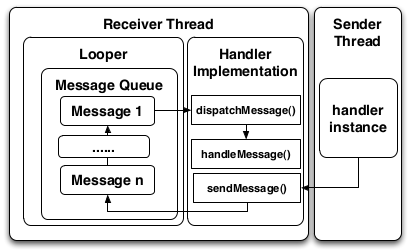
\includegraphics[width=0.7\linewidth]{looperHandler}
	\caption{Utilizzo di \texttt{Looper} e \texttt{Handler}}
	\label{fig:looperhandler}
\end{figure}
Figura~\ref{fig:looperhandler} mostra il funzionamento dei due costrutti. \texttt{Looper} si occupa di mantenere in un thread una coda di messaggi e di inviarli all'\texttt{Handler} opportuno, che li processerà. Il programmatore fornisce la logica per processare il messaggio implementando il metodo \texttt{handleMessage()} di \texttt{Handler}. Un'istanza di \texttt{Handler} è condivisa tra due thread per inviare e ricevere messaggi. Questo meccanismo è problematico quando più thread a priorità diverse inviano messaggi contemporaneamente. Ci sono due modi in cui i messaggi vengono processati. Di default l'ordine seguito è quello di ricezione. In aggiunta, però, un mittente può specificare un istante temporale nel quale il messaggio dovrà essere processato. In entrambi i casi però non viene considerata la priorità dei thread coinvolti. Se molti thread non real-time inviano simultaneamente messaggi allo stesso thread, insieme ad uno real-time, i messaggi di quest'ultimo saranno considerati solo dopo tutti i messaggi precedenti (Figura~\ref{fig:looperhandlerissue}). Inoltre, se altri thread non real-time inviano messaggi specificando un istante per processarli, la coda viene riordinata a run-time per fare in modo che questi messaggi vengano considerati in quel preciso istante. Questo significa che un thread real-time ad alta priorità può vedersi passare avanti un sacco di messaggi inviati da altri thread con una priorità molto più bassa.
\begin{figure}
	\centering
	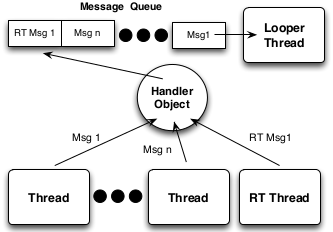
\includegraphics[width=0.7\linewidth]{looperHandlerissue}
	\caption{Scenario di ritardo per un thread real-time}
	\label{fig:looperhandlerissue}
\end{figure}

\subsubsection{Servizi di sistema}
L'implementazione di servizi come \texttt{SensorManager} o \texttt{AlarmManager}, utilizzati fortemente in applicazioni per il sensing dell'ambiente circostante, non tengono conto di eventuali vincoli temporali. 

\paragraph{AlarmManager.} Un'applicazione che vuole impostare un allarme invia un messaggio ad \texttt{AlarmManager}. Quando l'allarme scatta, all'istante specificato dall'applicazione, questa viene notificata e un metodo di callback, definito all'invio del primo messaggio, viene eseguito. Il problema è che non viene data nessuna garanzia sul tempo trascorso dallo scattare dell'allarme al momento in cui l'applicazione ne viene a conoscenza. 

\paragraph{SensorManager.}
Un'applicazione può ascoltare l'ambiente circostante attraverso le API di \texttt{SensorManager} e fornire delle callback. Queste vengono chiamate ogni volta che un evento di interesse si verifica. Ci sono due principali problemi: 
\begin{itemize}
	\item non c'è nessun supporto per le priorità dei thread, dato che tutti gli eventi finiscono nella stessa coda. Un thread ad alta priorità può dover aspettare un sacco di thread a priorità minore prima di ricevere i dati di cui ha bisogno;
	\item la consegna degli eventi avviene tramite uno scambio di messaggi tra tutte le classi coinvolte nel sensing. Android non fornisce nessuna garanzia sul tempo necessario a consegnare questi messaggi.
\end{itemize}
	\section{Panoramica di possibili diverse architetture per Android Real-Time}
\subsection{Proposte ad alto livello}
\begin{figure}[h]
	\centering
	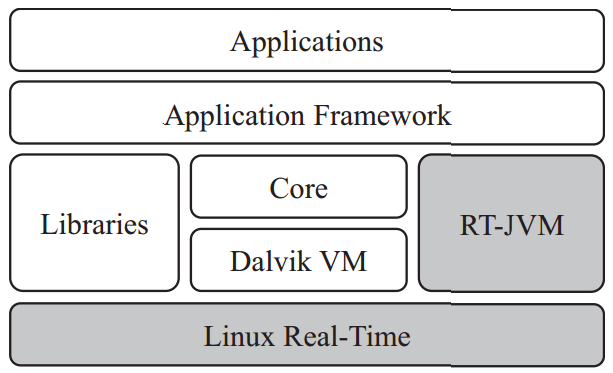
\includegraphics[width=0.7\linewidth]{androidPienoSupportoRT}
	\caption{Android Full real-time}
	\label{fig:androidpienosupportort}
\end{figure}
Una prima soluzione è mostrata in Figura~\ref{fig:androidpienosupportort} e considera la sostituzione di Linux con una versione real-time e l'aggiunta di una RT VM. Queste modifiche aggiungono prevedibilità e determinismo, ed è inoltre possibile aggiungere nuove politiche di scheduling attraverso le classi di scheduling e migliori strategie di gestione delle risorse. D'altra parte, però, tutti i driver utilizzati dal dispositivo devono essere implementati in un ottica real-time, e questo può portare a sforzi non necessari. La seconda modifica proposta riguarda l'aggiunta di una RT VM. Questa è considerata vantaggiosa, perché permette una gestione della memoria prevedibile. Inoltre, a seconda dell'algoritmo utilizzato, è anche possibile ottenere uno scheduling real-time, migliori meccanismi di sincronizzazione ed evitare l'inversione di priorità. Queste aggiunte sono assolutamente necessarie se si vuole ottenere una VM deterministica e prevedibile. Quest'ultima interagisce direttamente con il kernel per funzionalità come scheduling e gestione dei limiti di memoria. Non è necessario tenere il passo con le versioni di Android, perché è presente anche la DVM, ma è necessario implementare, la prima volta, una nuova Vm da zero e l'interprete Dalvik. Inoltre l'interazione di due VM può essere problematica, e può essere necessario pensare a nuovi algoritmi per ottimizzare lo scheduling.

\begin{figure}[h]
	\centering
	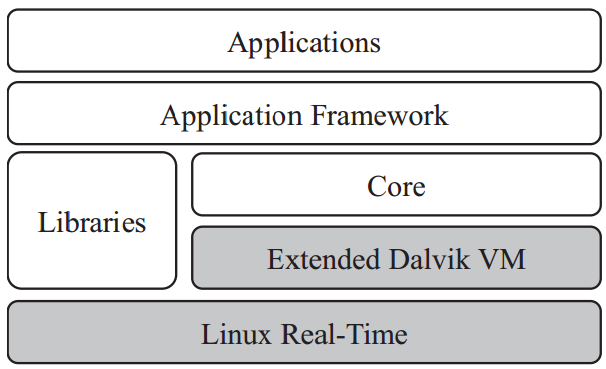
\includegraphics[width=0.7\linewidth]{androidEstesoRT}
	\caption{Android esteso con funzionalità real-time}
	\label{fig:androidestesort}
\end{figure}
La seconda soluzione è quella di sostituire Linux una versione real-time e di aggiungere funzionalità real-time a DVM (Figura~\ref{fig:androidestesort}). I vantaggi e gli svantaggi della sostituzione di Linux sono uguali a prima. Ora però la DVm viene estesa per supportare RTSJ. Questo permette di aggiungere alla DVm tutte le caratteristiche real-time previste dalla RTSJ, come GC real-time e gestione asincrona di eventi. In questo caso è però necessario stare al passo con i rilasci di nuove versioni della VM, per poter portare le modifiche a tutti i dispositivi Android.

\begin{figure}[h]
	\centering
	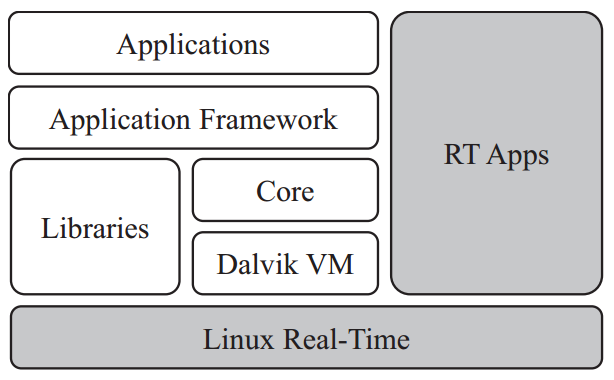
\includegraphics[width=0.7\linewidth]{rtandroidParziale}
	\caption{Android con support real-time parziale}
	\label{fig:rtandroidparziale}
\end{figure}
Il terzo approccio (Figura~\ref{fig:rtandroidparziale}) si basa ancora su Linux real-time e utilizza applicazioni real-time direttamente sopra il sistema operativo, utilizzando le librerie native. Questo è un vantaggio per quelle applicazioni che non necessitano della VM. Al contrario, però, le applicazioni che hanno bisogno della VM non possono avere supporto real-time.

\begin{figure}[h]
	\centering
	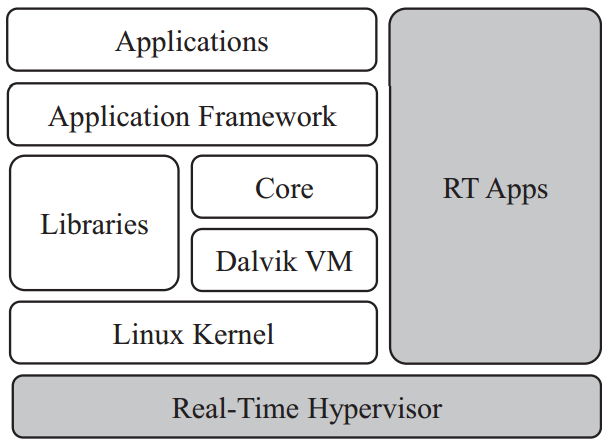
\includegraphics[width=0.7\linewidth]{androidConRTHypervisor}
	\caption{Android con real-time hypervisor}
	\label{fig:androidconrthypervisor}
\end{figure}
Il quarto approccio (Figura~\ref*{fig:androidconrthypervisor}) utilizza un real-time hypervisor in grado di eseguire parallelamente Android e applicazioni real-time. Questa soluzione è simile a quella utilizzata da alcuni sistemi operativi real-time, come RTLinux, e consiste nell'eseguire task real-time parallelamente (ma con priorità maggiore) a task del kernel. Lo svantaggio è che le applicazioni real-time godono delle sole funzionalità offerte dall'hypervisor, e quindi non possono utilizzare né i servizi della DVM né quelli di Linux. Inoltre, se un'applicazione real-time si blocca, l'intero sistema potrebbe bloccarsi.

\subsection{Liberare manualmente la memoria}
In \ref{sec:gcandroid} sono stati spiegate alcune criticità della GC in Android. Tuttavia, disabilitarla completamente non è una strada percorribile. Ogni processo ha la sua area di memoria e il GC viene invocato quando non c'è posto per soddisfare una richiesta di allocazione. Non liberare la memoria in questo contesto porterebbe sicuramente a comportamenti non prevedibili e distruttivi. Una soluzione più promettente potrebbe essere quella di liberare manualmente la memoria. In questo modo la probabilità che il GC sia invocato (e di conseguenza che l'applicazione venga bloccata) è minore. 

\begin{figure}[h]
	\centering
	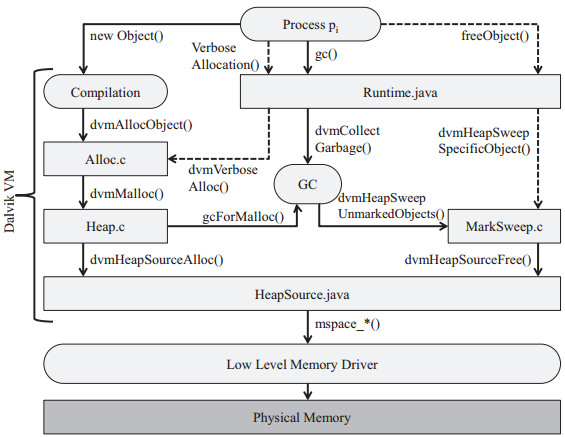
\includegraphics[width=0.7\linewidth]{../images/androidMemoryManagement}
	\caption{Gestione della memoria in Android}
	\label{fig:androidmemorymanagement}
\end{figure}

In Figura~\ref{fig:androidmemorymanagement} è mostrata la gestione della memoria in Android. Le transizioni rappresentano eventi di sistema, come chiamate di metodi, e mostrano i file sorgente coinvolti. I rettangoli arrotondati indicano entità astratte e componenti di sistema. Le linee tratteggiate rappresentano le estensioni proposte in questa soluzione. 

Durante la compilazione di un'applicazione Android, ogni istanziazione (\texttt{new}) viene tradotta in una chiamata a \texttt{dvmAllocObject()}. Questo metodo prende come argomento un riferimento alla classe richiesta. Tra le altre cose, questo riferimento contiene la dimensione dell'oggetto che si vuole creare. La dimensione viene passata a \texttt{dvmMalloc()}, che alloca la quantità di memoria desiderata. In generale, quest'ultima è responsabile della gestione degli errori, mentre l'allocazione vera e propria viene fatta da \texttt{dvmHeapSourceAlloc()}, che ritorna il risultato senza nessuna validazione. Se non ci sono errori, blocco viene poi convertito nell'oggetto e l'esecuzione continua. La chiamata può però fallire, ritornando un puntatore nullo e indicando la situazione della memoria. A questo punto \texttt{dvmMalloc()} prova a risolvere il problema avviando il GC,l dopodiché l'allocazione viene ripetuta o viene lanciata un'eccezione (\texttt{OutOfMemoryException}). Gli oggetti che non sono marcati dopo la passata del GC sono eliminabili. L'eliminazione viene fatta da \texttt{dvmHeapSweepUnmarkedObjects()}, che rilascia la memoria chiamando \texttt{dvmHeapSourceFree()} per ogni riferimento. Android offre anche la possibilità di richiedere esplicitamente la passata del GC, chiamando \texttt{Runtime.gc()} manualmente. Le chiamate esplicite al GC hanno gli stessi effetti negativi di quelle implicite. L'idea è quindi quella di pulire la memoria manualmente, oggetto per oggetto senza chiamare il GC. Sappiamo che \texttt{dvmHeapSourceFree()} offre la possibilità di eliminare un oggetto, dato il suo riferimento. Viene quindi aggiunto alla DVM un nuovo metodo, \texttt{dvmHeapSweepSpecificObject()}, che chiama \texttt{dvmHeapSourceFree()}. In più la classe \texttt{Runtime} viene estesa con il metodo \texttt{freeObject()}, per rendere disponibile la funzionalità per le applicazioni Android. \texttt{freeObject()} riceve come argomento un oggetto da rimuovere. Calcola il puntatore al blocco che contiene l'oggetto e lo passa a \texttt{dvmHeapSweepSpecificObject()}, che lo rimuove attraverso \texttt{dvmHeapSourceFree()}. Dopodiché la memoria è disponibile per un'altra allocazione. Uno svantaggio è che \texttt{freeObject()} può essere usato solo per quegli oggetti di cui lo sviluppatore è al corrente, ma la memoria può anche essere riempita di oggetti temporanei. Una soluzione è quella di aggiungere a \texttt{Runtime} anche il metodo \texttt{verboseAllocations()}, che permette di avere dei log su tutti gli oggetti che vengono allocati durante la vita di un processo. Questo log può poi essere usato per rendersi conto degli oggetti creati e liberare la memoria di conseguenza. 

\subsubsection{Valutazione}
In Figura~\ref{fig:valutazionegestionemanualememoria} viene mostrato un confronto fra la gestione della memoria manuale e con GC. Si nota che, raggiunti più o meno i 2900kB di memoria riferita, la DVM invoca il GC e l'applicazione viene, conseguentemente, bloccata. Al contrario, con la gestione manuale, il GC non viene mai invocato, perché la memoria riferita resta sempre sotto la soglia.
\begin{figure}[h]
	\centering
	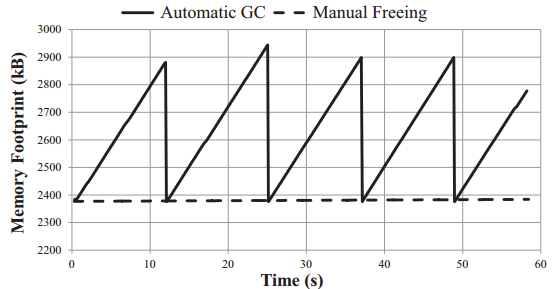
\includegraphics[width=0.7\linewidth]{valutazioneGestioneManualeMemoria}
	\caption{Valutazione della soluzione}
	\label{fig:valutazionegestionemanualememoria}
\end{figure}

Lo svantaggio e il limite evidente di questo approccio è che richiede che i programmatori gestiscano manualmente la memoria, proprio come in C o C++. Questo processo è estremamente difficoltoso, e può portare a molti leak e a gestioni scorrette. Sebbene prevenga l'invocazione del GC, gli errori introdotti dalla gestione manuale potrebbero portare l'applicazione ad un fallimento.
	\section{RTDroid - Versione base}
RTDroid si pone l'obiettivo di aggiungere supporto real-time ad Android nella sua interezza. Questo significa che tutti i problemi sopra riportati devono essere corretti in modo da fornire un supporto completo e che dia garanzie solide. In questa estensione, solamente un processo di livello utente (l'applicazione) è in esecuzione. 

Per risolvere tutti i problemi di Android è necessario un redesign profondo che arriva fino al livello del kernel. Quest'ultimo viene sostituito con un kernel real-rime, LinuxRT o, meglio, RTEMS. Anche la VM di Android viene sostituita, con Fiji. Sopra questo nuovo strato vengono offerte le ''classiche'' API Android, con l'aggiunta di una serie di estensioni che correggono specifici problemi riscontrati. Queste API aggiuntive rispettano la RTSJ. 

\subsection{Looper e Handler}
Ad ogni messaggio viene assegnata una priorità, attraverso due modalità:
\begin{itemize}
	\item\textit{inheritance}: il messaggio eredita la priorità del mittente;
	\item\textit{inheritance + specified}: il mittente può specificare una priorità relativa a tutti i messaggi inviati.
\end{itemize}
Dopodiché viene definita una coda per ogni priorità, con associata un \texttt{Looper} e un \texttt{Handler}. Messaggi a priorità più bassa non ritarderanno quelli a priorità più alta. Per avere garanzie sulla quantità di memoria utilizzata, le code possono essere dimensionate staticamente.

\subsection{AlarmManager}
Sia la registrazione che la consegna devono essere ridefinite per un completo supporto real-time. Per la registrazione vengono utilizzati degli alberi rosso neri (Figura~\ref{fig:rtalarm}), così da rendere il processo prevedibile sulla base della complessità delle operazioni sull'albero. 
\begin{figure}[h]
	\centering
	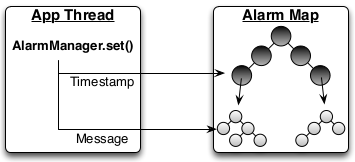
\includegraphics[width=0.6\linewidth]{rtalarm}
	\caption{Registrazione di allarmi real-time}
	\label{fig:rtalarm}
\end{figure}

L'albero principale mantiene i timestamp delle registrazioni e dei puntatori ad altri alberi, che ordinano i timestamp sulla base della priorità del richiedente. Di conseguenza una registrazione include solamente due inserimenti. Organizzando gli alberi in base alla priorità si ha la garanzia che un messaggio diretto ad un thread a bassa priorità non ritardi uno a priorità più alta. In questo modo, anche se un thread a bassa priorità registra un sacco di eventi (più di quanti ne possono essere gestiti), i thread a priorità più alta non verranno in nessun modo toccati.

Per la consegna viene definito un \texttt{AlarmManager} thread a cui è assegnata la priorità più alta di tutte. Questo thread sostituisce il classico meccanismo di invio di messaggi di Android. Si sveglia ogni volta che c'è un inserimento in un albero rosso nero e pianifica un thread all'istante temporale specificato. A quest'ultimo viene associata la callback specificata dall'applicazione.

\subsection{SensorManager}
Il sensing funziona attraverso un \textit{polling thread} che periodicamente ascolta l'ambiente circostante. Questo comunica con vari \textit{processing thread}, uno per ogni sensore, che interpretano i dati ricevuti dal polling thread.

I problemi riportati vengono risolti attraverso \textit{priority inheritance}. Quando un thread con priorità \texttt{p} registra un listener per un sensore, al thread associato a quel sensore viene assegnata la priorità \texttt{p}. Se più di un thread si associano allo stesso sensore, allora al thread del sensore è associata la priorità più alta tra tutti. Anche i thread creati per eseguire le callback hanno assegnata la priorità \texttt{p}. Il polling thread ha la priorità più alta di tutte, in modo da assicurare che i dati vengano raccolti appena possibile.

Quando un'applicazione registra un nuovo listener per un sensore viene di fatto creato un nuovo percorso di consegna dal polling thread al listener. Questo percorso è isolato ed eredita la priorità del thread che l'ha creato. 

\subsection{Sostituire componenti non real-time con componenti real-time}
Il kernel Linux di Android ha molte modifiche per renderlo adatto all'utilizzo in un ambiente con risorse limitate. Questo diventa un problema quando si cerca di sostituire alcuni componenti per migliorare il supporto real-time.

\paragraph{Bionic.} Un esempio è dato dalle librerie C native. Al posto di \texttt{glibc} Android utilizza \textit{Bionic}. Bionic è una libreria C leggera e altamente semplificata ed ottimizzata in modo da poter essere utilizzata in ambienti con risolrse limitate, in particolare CPU a bassa frequenza e poca memoria. Sfortunatamente però non aderisce alla specifica POSIX e non supporta le estensioni real-time di mutex e pthreads. Una modifica di questa libreria è necessaria per utilizzare una VM real-time, come Fiji.

\paragraph{Patch del kernel incompatibili.} Android ha introdotto molte modifiche al kernel Linux, tanto che l'applicazione automatica di patch per ottenere RTLinux è impossibile, e deve essere fatta manualmente. Anche dopo averla fatta manualmente, comunque, il kernel rimane non completamente prerilasciabile e questo comporta alti tempi di attesa possibili. 

\paragraph{Funzionalità non real-time del kernel.} Il kernel Android ha due funzionalità critiche sotto l'aspetto real-time. La prima è l'\textit{out of memory killer} (OOM), che viene avviato in condizioni di bassa memoria disponibile. Analizza tutte le pagine di memoria per verificare che il sistema sia veramente in condizioni critiche ed uccide un processo selezionato. I thread in esecuzione vengono fermati e bloccati per un periodo di tempo variabile. In un contesto dove è permessa solo l'esecuzione di un processo utente, però, OOM è inutile.

Un'altra funzionalità problematica è CPUFreq, che scala dinamicamente la frequenza della CPU. Android la usa per bilanciare le performance e la l'utilizzo della batteria. Il problema è che, quando CPUFreq cambia la frequenza, il cambiamento è percepito da tutti i thread running, introducendo jitter nel sistema. Inoltre il cambiamento non è tenuto in considerazione quando viene fatto lo scheduling, e quindi ci potrebbero essere deadline mancate e picchi di latenza non previsti. Esistono, comunque, scheduling real-time che tengono in considerazione i cambiamenti di voltaggio, e questi sono applicabili in questo contesto. Attualmente non ci sono soluzioni, ma una possibilità è considerare il caso peggiore (tutti i task nel loro caso peggiore e la peggiore frequenza possibile), anche se questo non considera il jitter del cambiamento di frequenza.

\section{RTDroid Migliorata}
La principale limitazione dell'approccio precedente è che viene data la possibilità di eseguire solo un processo utente per volta. Una seconda versione di RTDroid mira a risolvere questo problema, supportando l'esecuzione di più applicazioni real-time e non, come mostrato in Figura~\ref{fig:rtdroid}.

\begin{figure}[h]
	\centering
	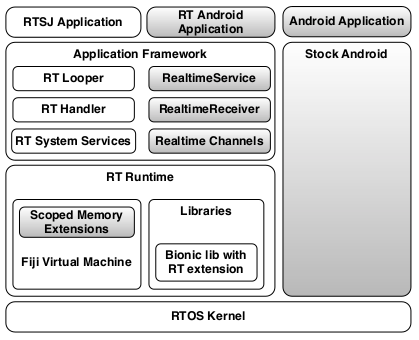
\includegraphics[width=0.6\linewidth]{rtdroid}
	\caption{RTDroid}
	\label{fig:rtdroid}
\end{figure}

Oltre ai cambiamenti introdotti precedentemente, RTDroid aggiunge costrutti real-time di alto livello, come (\textit{RealtimeService} e \textit{RealtimeReceiver}), costrutti di basso livello per la comunicazione (\textit{Realtime Channels}) e un meccanismo per specificare proprietà di questi costrutti. Le applicazioni senza vincoli temporali vengono eseguite in una VM separata. Questa modalità è utile anche per i componenti grafici delle applicazioni real-time. Figura\ref{fig:rtbootstrap} mostra il bootstrap.
\begin{figure}[h]
	\centering
	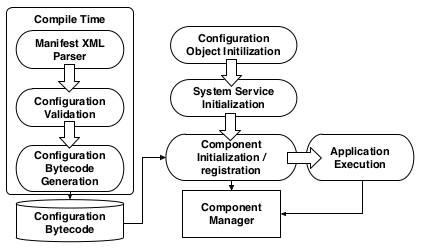
\includegraphics[width=0.6\linewidth]{rtbootstrap}
	\caption{Bootstrap di RTDroid}
	\label{fig:rtbootstrap}
\end{figure}

Quest'ultima è divisa in compile time e runtime. Il processo a due fasi assicura che la memoria possa essere pre allocata e che i componenti siano correttamente configurati. Durante la compilazione viene fatto il parsing del manifest, esegue dei controlli e genera il bytecode per la configurazione di tutti i componenti coinvolti. Questo bytecode rappresenta un gestore per ogni componente dell'applicazione. All'avvio, il sistema analizza la lista dei gestori e chiama quello appropriato per istanziare il componente corrispondente. Dopo l'istanziazione, il componente viene registrato presso un \textit{Component Manager}, che ne gestisce il ciclo di vita.

\subsection{Componenti}
RtDroid supporta tre diversi componenti real-time: \textit{services}, \textit{tasks} e \textit{receivers}. Un \texttt{RealtimeService} corrisponde ad un normale service Android, utilizzato per compiti aperiodici o sporadici. Dato che la nozione di computazione periodica non è presente in Android, viene introdotta la classe \texttt{PeriodicTask} per modellarla. \texttt{RealtimeReveiver}, invece, è usato per reagire ad eventi consegnati attraverso \texttt{Intent}. Non c'è bisogno di fornire un corrispettivo delle Activity. Queste ultime vengono utilizzate per la programmazione delle UI e possono essere eseguite senza vincoli temporali. L'interazione tra componenti real-time e non (UI) è permessa.

Ai componenti real-time viene assegnata una priorità, un tempo di inizio, una deadline e un limite di memoria. Questo viene fatto staticamente, estendendo i tag utilizzabili nel manifest.

Gestire il ciclo di vita dei componenti significa: 
\begin{enumerate}
	\item assicurare che priorità, deadline e periodicità;
	\item gestire automaticamente la memoria allocata;
	\item garantire che i limiti per ogni componente siano rispettati.
\end{enumerate}
Per (2) viene utilizzata un'allocazione basata sulle regioni. L'idea è di non gestire oggetti singoli, ma di allocare gli oggetti in regioni e poi operare al livello di una regione. L'idea è stata introdotta da RTSJ con le aree di memoria \textit{scoped}. I benefici principali sono due: i thread non devono essere bloccati durante la GC ed è possibile limitare il numero di regioni allocate da ciascun thread.

RTDroid supporta una forma semplificata di memoria scoped. Ogni componente ha accesso a due scope: \textit{Persistent Memory}, per dati la cui vita è legata al componente, e \textit{Release Memory}, che viene pulita prima di ogni rilascio di un componente periodico. La dimensione di queste aree è definita nel manifest. La memoria totale assegnata ad un componente è la somma di peristent memory, release memory e memoria assegnata ai sotto-componenti.

\paragraph{Service} \mbox{} \\
Un service real-time è una classe astratta e un programmatore deve implementare le sue callback. Queste sono ereditate direttamente da \texttt{Service} di Android e vengono invocati nei diversi stadi del ciclo di vita. Contrariamente ad Android, che esegue i service nello stesso thread della UI, RTDroid li esegue in thread separati (mappati con i thread real-time della JVM sottostante), in modo da supportare diverse priorità. Quando viene inizializzato, ad un service viene assegnata una persistent memory che ha lo stesso tempo di vita del service stesso (allocato allo start e deallocato alla terminazione). Inoltre, se vengono utilizzati dei canali di comunicazione, le code per gli intent sono allocate nella persistent memory. Oltre ai task periodici, anche le callback eseguono utilizzando la release memory, che viene pulita al termine dell'esecuzione. La struttura è mostrata in Figura~\ref{fig:scopeservice}.

Il manifest deve dichiarare quanta memoria è richiesta, in modo da dimensionare in modo corretto.
\begin{figure}[h]
	\centering
	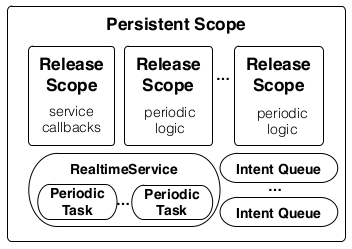
\includegraphics[width=0.6\linewidth]{scopeService}
	\caption{Struttura dello scope per un Service}
	\label{fig:scopeservice}
\end{figure}

\paragraph{Task periodici}\mbox{} \\
Un task periodico è un sotto-componente di un service. Oltre alle caratteristiche del parent, un task ha bisogno di un periodo.

\paragraph{Receiver}\mbox{} \\
In Android, un nuovo broadcast receiver viene allocato ogni volta che un intent è ricevuto. Se tanti intent vengono inviati ad un componente, il risultato è una frequente allocazione/deallocazione. In RTDroid, invece, un receiver real-time è un costrutto persistente, e viene riutilizzato per ridurre l'impatto sulla memoria. Come conseguenza diretta,un receiver può processare un solo intent alla volta, e la logica dell'applicazione è espressa a callback. In \texttt{onReceive()} va specificato come si reagisce aglie eventi, mentre \texttt{onClean()} è usato per pulire la memoria. La sua implementazione è necessaria se si desidera avere una gestione stateless degli eventi, ed è non necessaria se vengono modificate solo variabili locali che risiedono nella release memory, che viene pulita automaticamente).

Un'importante scelta progettuale riguarda la priorità delle callback. Queste vengono eseguite alla stessa priorità dei loro componenti. Callback multiple generate da una serie di intent sono eseguite in ordine. Dal punto di vista implementativo eusto significa che un receiver è collegato ad un gestore di eventi asincrono nella JVM, che gestisce le ricezioni con una coda a priorità. Questo assicura che messaggi provenienti da mittenti ad alta priorità verranno consegnati prima. 

\subsection{Comunicazione}
RTDroid fornisce quattro tipi di canali real-time:
\begin{itemize}
	\item message;
	\item broadcast;
	\item trasferimento di grandi quantità di dati;
	\item cross-context, per comunicare ocn componenti non real-time.
\end{itemize}
I programmatori devono specificare il nome del canale, il tipo di dato trasferito e la sua dimensione. Inoltre, i componenti real-time devono specificare il numero di messaggi che invieranno e riceveranno nel corso della loro vita. Questo assicura la possibilità di preallocare gli oggetti corrispondenti ai messaggi e di tenere sotto controllo i limiti di memoria per ciascun componente. Di questi quattro canali, i primi tre devono esplicitamente essere creati dai programmatori, mentre ne esiste uno predefinito per la comunicazione con i componenti non real-time.

Ogni canale deve specificare (nel manifest) il suo comportamento a runtime come segue: tipo, ordine di ricezione dei messaggi, priorità dell'esecuzione della callback associata e politica di cancellazione, tipo e dimensione dei dati. I compoennti possono utilizzare \texttt{intent-filter} per identificarsi come publishers o subscribers e specificare il numero di messaggi letti o inviati in ogni rilascio della callback. 

Il principale beneficio dell'utilizzo del manifest è che c'è un controllo statico. RTDroid garantisce la correttezza dell'applicazione in due aspetti:
\begin{itemize}
	\item check dei limiti di memoria: la memoria richiesta da un componente deve essere uguale alla somma di persistent, release e memoria dei sotto-componenti;
	\item check di channel overflow: il tasso di messaggi in entrata non dovrebbe eccedere il limite dei messaggi processabili da quel canale.
\end{itemize}

\paragraph{Message channels} \mbox{} \\
Un canale di questo tipo ha tre caratteristiche principali:
\begin{enumerate}
	\item il \texttt{RealtimeHandler} associato deve essere registrato un un service real-time;
	\item possono essere scambiati solo array di tipi primitivi o buffer di byte a lunghezza fissa;
	\item il numero di messaggi in attesa è limitato.
\end{enumerate}

RTDroid crea una coda a dimensione fissa per ogni canale. Anche i messaggi sono preallocati, e vivono nella persistent memory del destinatario. Figura~\ref{fig:messagechannel} mostra la gerarchia nella memoria scoped.
\begin{figure}[h]
	\centering
	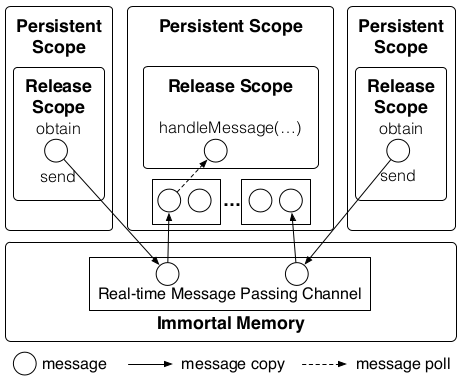
\includegraphics[width=0.6\linewidth]{messageChannel}
	\caption{Real-time message channels}
	\label{fig:messagechannel}
\end{figure}

L'accodamento dei messaggi è gestito alla priorità del mittente, mentre l'estrazione è gestita alla priorità del destinatario. Se la coda è piena, un componente ad alta priorità può rubare un messaggio ad un mittente con bassa priorità. Quando questo accade, il componente ad alta priorità sarà in grado di accodare il messaggio, mentre quello a bassa priorità riceverà un'eccezione.

L'invio è difficoltoso perché i messaggi sono preallocati e i mittenti non dovrebbero mantenere riferimenti ai messagi dopo che questi sono stati inviati. Il protocollo usato è quindi indiretto. Una \texttt{MessageClosure} è allocata dal mittente, e la callback \texttt{getMsg()} è usata per popolare il payload.

Il riferimento al messaggio viene dato in base alla priorità del mittente. Di conseguenza l'operazione può fallire se non ci sono messaggi con quella priorità (sono tutti in uso). In questo caso viene lanciata un'eccezione. Se un componente ad alta priorità cerca di ottenere un messaggio, ma sono tutti utilizzati, può rubare un messaggio correntemente in uso da un componente non real-time a priorità più bassa. Dato che tutti i messaggi sono ottenuti durante il metodo \texttt{send} di \texttt{MessageClosure}, tutti i messaggi in uso corrispondono a messaggi accodati, ma non ricevuti. Se il messagio viene rubato viene sollevata un'eccezione asincrona, utilizzando il meccanismo \texttt{AsynchronousInterruptedException} previsto da RTSJ.

Una volta che un messaggio viene ottenuto, il mittente deve copiare i dati da inviare dal suo spazio di memoria allo spazio del canale.Questo assicura che un mittente non possa utilizzare o riempire lo spazio del destinatario direttamente, ma quest'ultimo deve accettare la ricezione. Una volta che il messaggio è copiato dall'handler del destinatario, l'oggetto del messaggio è rimesso nel pool. Questa strategia mantiene costante l'ammontare di memoria dedicata al passaggio dei messaggi. Il mittente deve utilizzare la sua memoria per memorizzare i dati che vuole inviare e non può usare le risorse del sistema finché non gli viene concesso il messaggio.

\paragraph{Broadcast Channel} \mbox{} \\
Questi canali sono usati per invocare callback in componenti real-time, disaccoppiando la priorità della consegna dell'intent dall'invocazione delle callback. La differenza tra messaggi e intent è che i primi hanno un solo destinatario, mentre i secondi no e per riceverli bisogna esplicitarlo nel manifest. 

\begin{figure}[h]
	\centering
	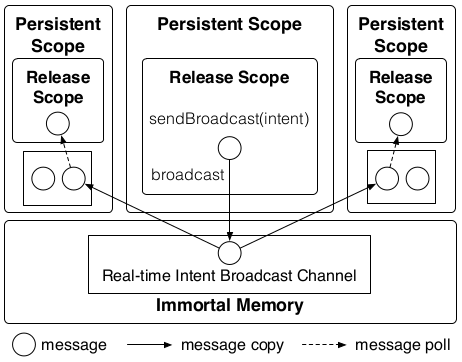
\includegraphics[width=0.6\linewidth]{images/broadcastChannel}
	\caption{Real-time broadcast channels}
	\label{fig:broadcastchannel}
\end{figure}

Figura~\ref{fig:broadcastchannel} mostra come un intent persiste nella memoria immortal fino a quando non è copiato in tutte le code dei subscribers. Sebbene il messaggio sia replicato per ogni subscriber, solo una copia è salvata nel canale. Il numero di destinatari è salvato in un contatore, e viene decrementato ad ogni ricezione. L'ultimo destinatario rilascia il messaggio e lo rimette nel pool, esattamente come nei message channels. L'utilizzo di memoria è limitato.

\paragraph{Bulk Data Channels} \mbox{} \\
Questo canale permette di trasferire dati di grandi dimensioni senza copiarli. Per supportarli viene esteso il concetto di memoria annidata con quello di memoria annidata trasferibile. Uno scope, che incapsula i dati, vene rimosso dallo stack del mittente e messo nello stack del destinatario. Di conseguenza, il mittente non può né allocare né scrivere dati in quello scope. L'idea funziona solo se il frame è il primo nello stack e se lo stack è lineare. Dato che gli scopes non sono esposti ai programmatori, i vincoli sono rispettati per costruzione dalla struttura del canale. In parole povere, quindi, questi canali permettono al mittente di creare uno scope trasferibile, di popolarlo con i dati, e di cederne l'accesso.

\paragraph{Cross-Context Channels} \mbox{} \\
Questi canali permettono alle Activities di comunicare con i componenti real-time. La comunicazione avviene tra due diverse VM, una delle quali esegue codice non real-time e RTDroid, che esegue applicazioni real-time. In questo modo si può interagire sia con il sistema Android che con le altre applicazioni. Al fine di questa comunicazione un'applicazione deve dichiarare un service, \texttt{RTsProxyService}, che sottoscrive un canale dichiarato in un'applicazione real-time. Nell'altra direzione, un'applicazione real-time si deve solo sottoscrivere agli intent che l'applicazione non real-time ha dichiarato nel suo manifest. Il service proxy permette al codice non real-time di inviare messaggi ai componenti real-time. Per limitare la memoria il numero di intent in un canale è limitato e ogni intent ha un payload di lunghezza fissata.
\begin{figure}[h]
	\centering
	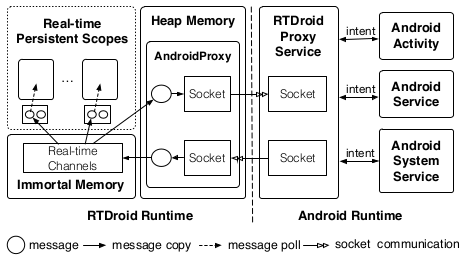
\includegraphics[width=0.6\linewidth]{crosscontentChannel}
	\caption{Cross-Content channel}
	\label{fig:crosscontentchannel}
\end{figure}

Figura~\ref{fig:crosscontentchannel} mostra come la comunicazione bidirezionale viene stabilita attraverso sockets. Vengono usati due componenti proxy in ogni runtime. Per evitare interferenza, il proxy di Android è eseguito sullo heap ed esegue ad una priorità real-time bassa. I messaggi in arrivo sono tradotti in intent o messaggi real-time con la più bassa priorità e inviati (attraverso canali real-time) ai componenti opportuni. In questi canali viene depositato solo un messaggio alla volta, in modo da evitare che componenti non real-time esauriscano la memoria usata da quelli real-time. I primi possono esaurire lo heap, ma questo non ha nessuna ripercussione sui secondi, che usano regioni preallocate.

\subsection{Gestione della memoria}
Fornire garanzie sulla memoria implica che il sistema sottostante deve fornire un'allocazione prevedibile (cioè l'allocazione degli oggetti non deve essere bloccata dal fatto che qualcun altro sta usando la memoria) e una reclamazione prevedibile (la gestione della memoria non deve interferire con l'esecuzione di componenti real-time). Per entrambi si usa la scoped memory, che fornisce una quantità fissa di memoria per task real-time con allocazione e deallocazione prevedibili. In aggiunta, la memoria scoped assicura che i thread real-time non siano bloccati durante la GC (se usano solo scoped memory). Come già detto, la RTSJ prevede tre tipi di memoria: 
\begin{itemize}
	\item heap, che è garbage collected;
	\item immortal, mai reclamata;
	\item scoped, fornisce regioni di dimensione fissa.
\end{itemize}
Per garantire l'integrità dei riferimenti RTSJ impone un'insieme di regole sulla gestione della scoped memory, ad esempio:
\begin{itemize}
	\item gli oggetti in uno scope sono reclamati solo quando tutti i thread in quello scope sono terminati;
	\item ogni thread deve entrare in uno scope sempre dallo stesso parent scope;
	\item uno scope con un tempo di vita lungo non può mantenere un riferimento ad un oggetto allocato in uno scope con un periodo di vita più corto. 
\end{itemize}

Le esecuzioni di componenti e callback (e le allocazioni associate) vengono separate per fornire un limite alla memoria occupata da ciascun componente. Il ciclo di vita di un componente viene gestito nel persistent scope (persistent memory), mentre l'invocazione delle callbacks viene gestita nel release scope (release memory). Ogni componente è legato ad un thread di controllo che è avviato nell'immortal memory. Questo assicura che la memoria necessaria per creare il contesto di esecuzione sia sempre disponibile. La stessa cosa vale anche per i canali di comunicazione.

\subsection{Valutazione}
\subsubsection{Micro Benchmark dei canali}
Il test vede due servizi real-time (alta priorità) che si scambiano messaggi (un sender e un receiver) ogni 100ms e uno non real-time che genera rumore (bassa priorità). Quest'ultimo esegue nello heap e fa partire 30 thread che disturbano lo scambio di messaggi. Questi thread sono di tre tipi:
\begin{itemize}
	\item heap noise, allocano un array di 512 byte nello heap ogni 200ms;
	\item computational noise, calcolano $\pi$ ogni 200ms;
	\item message noise, inviano un messaggio a bassa priorità al service receiver ogni 200ms.
\end{itemize}

Figura~???? mostra le misurazioni delle prestazioni. Lo scambio di messaggi consiste nell'allocazione del messaggio (da parte del mittente), nella sua consegna e nel context switch mittente/destinatario. Figura~??? mostra la situazione con solo mittente e destinatario, e serve per i confronti. Viene mostrata la latenza per 2000 eventi generati dallo scambio dei messaggi. Per ogni evento si definisce:
\begin{itemize}
	\item \textbf{message allocation latency}: tempo necessario per istanziare un messaggio;
	\item \textbf{message passing latency}: tempo necessario per la consegna;
	\item \textbf{context switch latency}: tempo trascorso tra l'invio del messaggio e il momento in cui questo viene processato.
\end{itemize}
I tre tipi di latenza sono strettamente limitati per tutti gli eventi, senza nessun punto anomalo che si discosta fortemente dagli altri. Senza nessun sovraccarico, questa architettura è stabile e prevedibile.

Un esperimento simile viene fatto con gli intents. Il mittente invia un intent ogni 100ms, e il receiver esegue una callback che, semplicemente, risponde al messaggio. Si definiscono:
\begin{itemize}
	\item \textbf{intent delivery latency}: latenza complessiva per ogni intent;
	\item \textbf{callback trigger latency}: tempo richiesto per generare una nuova callback.
\end{itemize}
I risultati sono mostrati in Figura~???, e sono simili a quelli precedenti.

Allo stesso modo, Figura~??? mostra la baseline per il trasferimento di dati di grosse dimensioni. La \textbf{transfer latency} è il tempo di consegna di un intent con un payload molto pesante.

Figura~??? mostra i grafici CDF (cumulative distribution function) che confrontano le prestazioni dei tre tipi di canali. In particolare, i CDF illustrano che percentuale dei punti misurati è minore o uguale di un certo valore temporale. Per il messaging (Figura~???), indipendentemente dal carico a cui è sottoposto, RTDroid si comporta bene (non ci sono grossi cambiamenti di latenza). Sebbene i risultati siano simili per gli intents (Figura~???), si nota un overhead maggiore rispetto al messaging semplice. Questo era prevedibile, dato che l'intent è associato all'esecuzione di una callback. Figura~??? mostra i risultati per il trasferimento di dati di diverse dimensioni. RTDroid praticamente non risente del cambiamento di dimensioni (giustamente, perché non fa nessuna copia dei dati).

\subsection{Confronto con Android e con RTSJ}



	
	
	%bibliography
	\newpage
	\nocite{*}
	\printbibliography 
	
\end{document}